% Basel problem visualization - bar chart
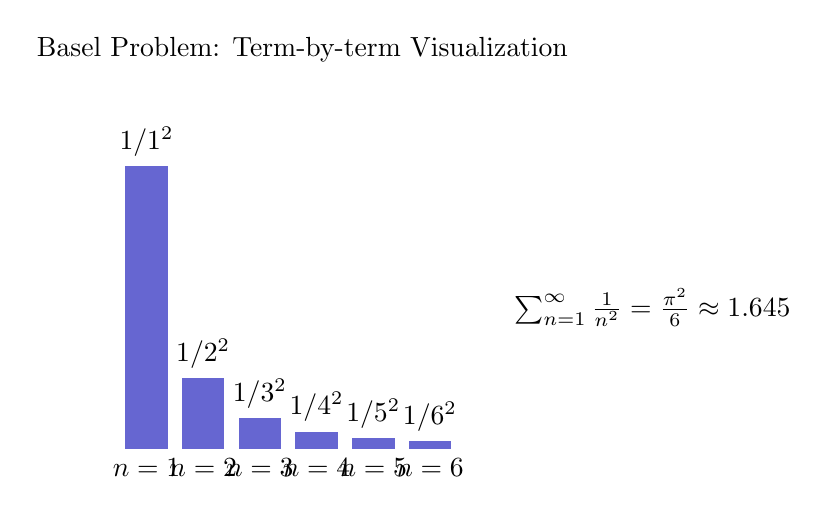
\begin{tikzpicture}[scale=0.9]
  % Bars showing 1/n^2
  \def\maxh{4}
  \foreach \n/\h in {1/\maxh, 2/1, 3/0.44, 4/0.25, 5/0.16, 6/0.11} {
    \fill[blue!70!black!60] (\n*0.8-0.3,0) rectangle (\n*0.8+0.3,\h);
    \node[below] at (\n*0.8,0) {$n=\n$};
    \node[above] at (\n*0.8,\h) {$1/\n^2$};
  }
  
  % Sum annotation
  \node[right=0.5cm] at (6*0.8+0.5,2) {$\sum_{n=1}^{\infty} \frac{1}{n^2} = \frac{\pi^2}{6} \approx 1.645$};
  
  % Title
  \node[above=0.3cm] at (3,5) {Basel Problem: Term-by-term Visualization};
\end{tikzpicture}
